% Created 2020-08-14 Fri 20:37
% Intended LaTeX compiler: pdflatex
\documentclass[11pt]{article}
\usepackage[utf8]{inputenc}
\usepackage[T1]{fontenc}
\usepackage{graphicx}
\usepackage{grffile}
\usepackage{longtable}
\usepackage{wrapfig}
\usepackage{rotating}
\usepackage[normalem]{ulem}
\usepackage{amsmath}
\usepackage{textcomp}
\usepackage{amssymb}
\usepackage{capt-of}
\usepackage{hyperref}
\usepackage{minted}
\usepackage{/home/ryan/Dropbox/profiles/Templates/LaTeX/ScreenStyle}
\author{Ryan Greenup}
\date{\today}
\title{Big Data; 04 Practical - MongoDB Basics}
\hypersetup{
 pdfauthor={Ryan Greenup},
 pdftitle={Big Data; 04 Practical - MongoDB Basics},
 pdfkeywords={},
 pdfsubject={},
 pdfcreator={Emacs 27.1 (Org mode 9.4)}, 
 pdflang={English}}
\begin{document}

\maketitle
\tableofcontents

\section{Using the \texttt{product} Database}
\label{sec:org6fad599}
The \url{./product.json} Database will be used here
\subsection{Using the Mongo-compass program\hfill{}\textsc{ATTACH}}
\label{sec:org4b889ba}
\begin{enumerate}
\item Open mongo-compass

\item Connect to the mongoDB server

\begin{enumerate}
\item Probably localhost:27017

\begin{enumerate}
\item If you're on SystemD maybe check with \texttt{sudo systemctl status mongodb}, for me I got a different port number.
\end{enumerate}

\begin{center}
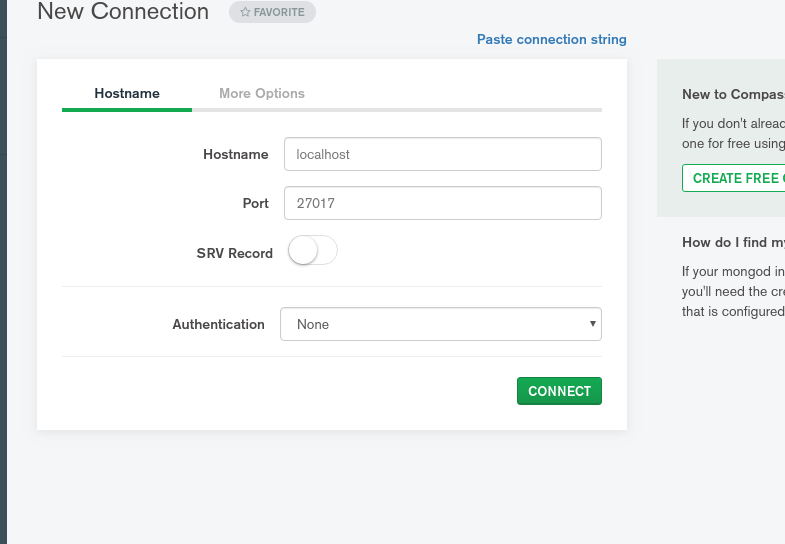
\includegraphics[width=.9\linewidth]{org-compass-Server.png}
\end{center}
\end{enumerate}

\item Create a new collection

\begin{center}
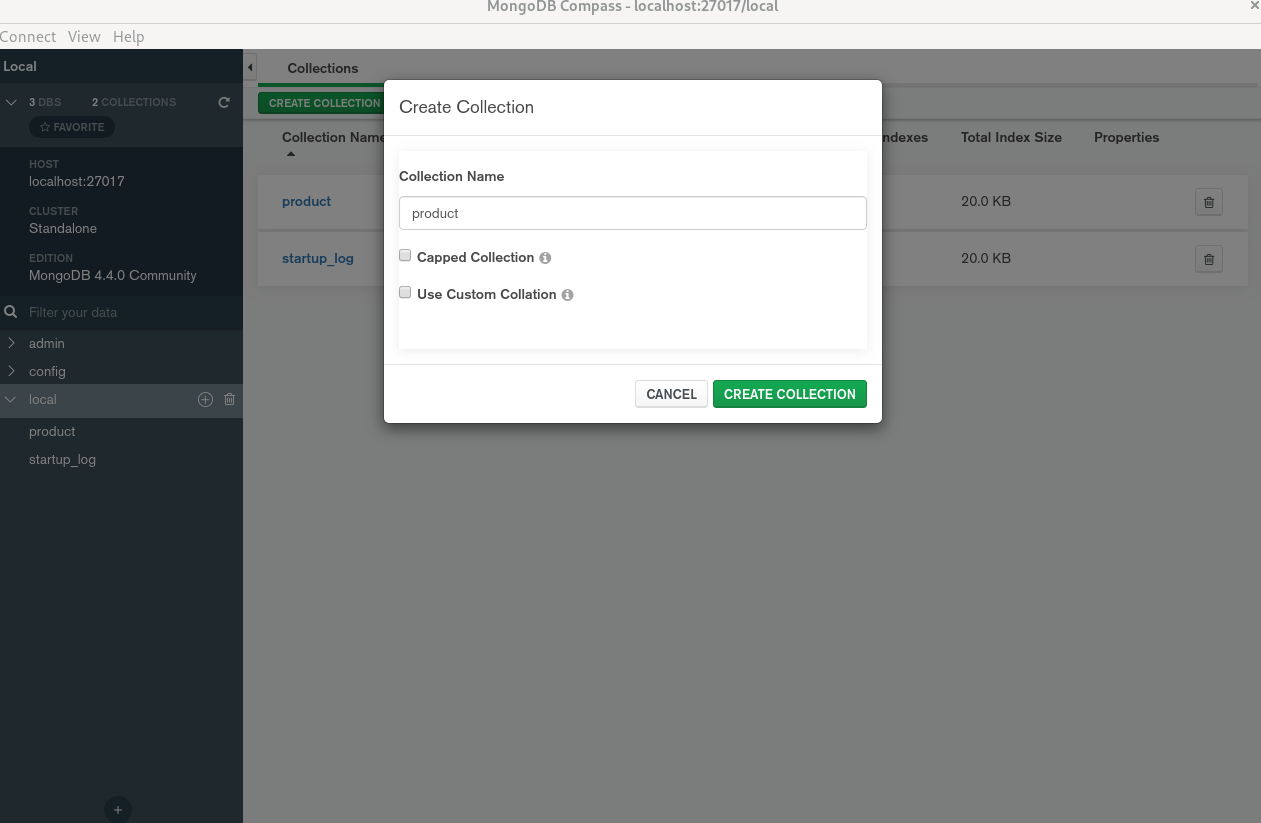
\includegraphics[width=.9\linewidth]{org-compass-Collection.png}
\end{center}

\item Import the JSON File

\item Now from the terminal run \texttt{mongo} to open a shell and then \texttt{use local} to switch to that database.
\end{enumerate}

\subsection{List Movies}
\label{sec:orga8ff286}
First see if you can list everything, if you created product underneath local, you'll need to do something like this:

\begin{minted}[]{javascript}
use local
db.product.find()
\end{minted}

In the case of \url{./product.json}, the following should return some output.

\begin{minted}[]{javascript}
db.product.find({'Type': 'Movie'})
\end{minted}

\begin{minted}[]{json}
{ "_id" : ObjectId("551668dbeb88341eb801f2d2"), "Classification" : "PG-13", "Title" : "Inception", "Price" : { "Buy" : 9.99, "Rent" : 2.99 }, "Director" : "Christopher Nolan", "Cast" : [ "Leonardo DiCaprio", "Joseph Gordon-Levitt" ], "Year" : "2010", "Genre" : [ "Drama", "Action", "Science Fiction" ], "Type" : "Movie", "Length (min)" : 148 }
{ "_id" : ObjectId("551668dbeb88341eb801f2db"), "Classification" : "R", "Title" : "Superbad", "Price" : { "Buy" : 9.99, "Rent" : 2.99 }, "Director" : "Greg Mottola", "Cast" : [ "Jonah Hill", "Michael Cera" ], "Year" : "2007", "Genre" : "Comedy", "Type" : "Movie", "Length (min)" : 113 }
{ "_id" : ObjectId("551668dbeb88341eb801f2dc"), "Title" : "Dracula", "Price" : { "Buy" : 9.99, "Rent" : 3.99 }, "Director" : "Tod Browning", "Cast" : [ "Bela Lugosi", "Helen Chandler" ], "Year" : "1931", "Genre" : [ "Classics", "Horror" ], "Type" : "Movie", "Length (min)" : 75 }

...
...
...
\end{minted}

To query all the text, something like this might be useful:

\begin{minted}[]{bash}
mongo --eval 'db.product.find()' local | fzf
\end{minted}

To return All Movies that contain, for example, Morgan Freeman, Compass can be inspected to reveal the \texttt{cast} field and then the following can be used:
\begin{minted}[]{javascript}
db.product.find({'Cast': 'Morgan Freeman'})
\end{minted}

\begin{minted}[]{json}
{ "_id" : ObjectId("551668dbeb88341eb801f2de"), "Title" : "The Shawshank Redemption" }
{ "_id" : ObjectId("551668dbeb88341eb801f2e7"), "Title" : "The Dark Knight" }
> db.product.find({'Cast': 'Morgan Freeman'})
{ "_id" : ObjectId("551668dbeb88341eb801f2de"), "Classification" : "R", "Title" : "The Shawshank Redemption", "Price" : { "Buy" : 9.99, "Rent" : 3.99 }, "Director" : "Frank Darabont", "Cast" : [ "Tim Robbins", "Morgan Freeman" ], "Year" : "1994", "Genre" : "Drama", "Type" : "Movie", "Length (min)" : 142 }
{ "_id" : ObjectId("551668dbeb88341eb801f2e7"), "Classification" : "PG-13", "Title" : "The Dark Knight", "Price" : { "Buy" : 12.99, "Rent" : 3.99 }, "Director" : "Christopher Nolan", "Cast" : [ "Christian Bale", "Heath Ledger", "Morgan Freeman" ], "Year" : "2008", "Genre" : [ "Drama", "Action", "Science Fiction" ], "Type" : "Movie", "Length (min)" : 152 }
>
\end{minted}

This however returns too much information, instead we can use \href{https://docs.mongodb.com/manual/tutorial/project-fields-from-query-results/}{projection} to filter the results:

\begin{minted}[]{javascript}
db.product.find({'Cast': 'Morgan Freeman'}, {Title: 1})
\end{minted}

\begin{minted}[]{json}
{ "_id" : ObjectId("551668dbeb88341eb801f2de"), "Title" : "The Shawshank Redemption" }
{ "_id" : ObjectId("551668dbeb88341eb801f2e7"), "Title" : "The Dark Knight" }
\end{minted}

\subsection{Find Songs}
\label{sec:org2e247c6}

To Find the Songs in the Database the following can be used:

\begin{minted}[]{javascript}
db.product.find({'Type': 'Song'})
\end{minted}

This returns far too many results, so instead projection can be used:

\begin{minted}[]{javascript}
db.product.find({'Type': 'Song'}, {'Title': 1, })
\end{minted}

\begin{minted}[]{json}
{ "_id" : ObjectId("551668dbeb88341eb801f2d3"), "Title" : "Someone Like You" }
{ "_id" : ObjectId("551668dbeb88341eb801f2d5"), "Title" : "Billie Jean" }
{ "_id" : ObjectId("551668dbeb88341eb801f2d6"), "Title" : "Speak to Me" }
{ "_id" : ObjectId("551668dbeb88341eb801f2d7"), "Title" : "I Will Always Love You" }
{ "_id" : ObjectId("551668dbeb88341eb801f2d9"), "Title" : "Back in Black" }
{ "_id" : ObjectId("551668dbeb88341eb801f2df"), "Title" : "2 Becomes 1" }
{ "_id" : ObjectId("551668dbeb88341eb801f2e2"), "Title" : "Enter Sandman" }
{ "_id" : ObjectId("551668dbeb88341eb801f2e4"), "Title" : "Smells Like Teen Spirit" }
{ "_id" : ObjectId("551668dbeb88341eb801f2e6"), "Title" : "Yesterday" }
{ "_id" : ObjectId("551668dbeb88341eb801f2e9"), "Title" : "When You Believe" }
\end{minted}

In order to filter by Genre we could just add that to the \texttt{find} field, however because we want any type of rock, we'll need to use the \texttt{.*Rock.*} regex, this has an odd syntax in \emph{MongoDB} where a regex term is denoted like this: \texttt{\{ \$regex: /.*Rock.*/ \}}, so putting that together:

\begin{minted}[]{javascript}
db.product.find({'Type': 'Song', 'Genre': { $regex: /.*Rock.*/ }}, {'Title': 1, 'Artist': 1, 'Album': 1})
\end{minted}

\begin{minted}[]{json}
{ "_id" : ObjectId("551668dbeb88341eb801f2d5"), "Album" : { "Certification" : "43xPlatinium", "Title" : "Thriller" }, "Artist" : "Michael Jackson", "Title" : "Billie Jean" }
{ "_id" : ObjectId("551668dbeb88341eb801f2d6"), "Album" : { "Certification" : "23xPlatinium", "Title" : "The Dark Side of the Moon" }, "Artist" : "Pink Floyd", "Title" : "Speak to Me" }
{ "_id" : ObjectId("551668dbeb88341eb801f2d9"), "Album" : { "Certification" : "26xPlatinium", "Title" : "Back in Black" }, "Artist" : "AC/DC", "Title" : "Back in Black" }
{ "_id" : ObjectId("551668dbeb88341eb801f2e4"), "Album" : { "Certification" : "17xPlatinium", "Title" : "Nevermind" }, "Artist" : "Nirvana", "Title" : "Smells Like Teen Spirit" }
{ "_id" : ObjectId("551668dbeb88341eb801f2e6"), "Album" : { "Certification" : "22xPlatinium", "Title" : "1" }, "Artist" : "The Beatles", "Title" : "Yesterday" }
\end{minted}

To sort thhe results, the \texttt{.sort()} method can be tacked on the end like so:

\begin{minted}[]{javascript}
db.product.find({'Type': 'Song', 'Genre': { $regex: /.*Rock.*/ }}, {'Title': 1, 'Artist': 1, 'Album': 1}).sort({ 'ReleaseDate': -1 })
\end{minted}

\begin{minted}[]{json}
{ "_id" : ObjectId("551668dbeb88341eb801f2e6"), "Album" : { "Certification" : "22xPlatinium", "Title" : "1" }, "Artist" : "The Beatles", "Title" : "Yesterday" }
{ "_id" : ObjectId("551668dbeb88341eb801f2e4"), "Album" : { "Certification" : "17xPlatinium", "Title" : "Nevermind" }, "Artist" : "Nirvana", "Title" : "Smells Like Teen Spirit" }
{ "_id" : ObjectId("551668dbeb88341eb801f2d5"), "Album" : { "Certification" : "43xPlatinium", "Title" : "Thriller" }, "Artist" : "Michael Jackson", "Title" : "Billie Jean" }
{ "_id" : ObjectId("551668dbeb88341eb801f2d9"), "Album" : { "Certification" : "26xPlatinium", "Title" : "Back in Black" }, "Artist" : "AC/DC", "Title" : "Back in Black" }
{ "_id" : ObjectId("551668dbeb88341eb801f2d6"), "Album" : { "Certification" : "23xPlatinium", "Title" : "The Dark Side of the Moon" }, "Artist" : "Pink Floyd", "Title" : "Speak to Me" }
>
\end{minted}
\subsection{Calculate the Average Price of Books}
\label{sec:org4e179ed}

To find all books with more than 500 pages, the \href{https://docs.mongodb.com/manual/tutorial/query-documents/}{And} operator can be used inside \texttt{find}, this amounts to just using a \texttt{,}.

Operators are, much like regex, a little odd, they require cages and \texttt{\$} prefixes.

\begin{minted}[]{javascript}
 db.product.find( { 'Type': 'Book', Pages: { $gt: 500 } } )
\end{minted}

\begin{minted}[]{json}
{ "_id" : ObjectId("551668dbeb88341eb801f2d0"), "Publisher" : "Prentice Hall", "ISBN" : "132126958", "Author" : "Andrew Tanenbaum", "Price" : 129.79, "Title" : "Computer Networks", "Shipping" : { "Weight (lb)" : 2.9, "Dimension (in)" : { "Width" : 6.6, "Depth" : 1.5, "Height" : 9.2 } }, "Edition" : "5", "Year" : "2010", "Type" : "Book", "Pages" : 960 }
{ "_id" : ObjectId("551668dbeb88341eb801f2d4"), "Publisher" : "Pearson", "ISBN" : "032182573X", "Author" : "Peter Tanenbaum", "Price" : 153.16, "Title" : "Excursions in Modern Mathematics", "Shipping" : { "Weight (lb)" : 3.2, "Dimension (in)" : { "Width" : 8.8, "Depth" : 1.1, "Height" : 10.9 } }, "Edition" : "8", "Year" : "2012", "Type" : "Book", "Pages" : 608 }
{ "_id" : ObjectId("551668dbeb88341eb801f2e0"), "Publisher" : "Prentice Hall", "ISBN" : "013359162X", "Author" : "Andrew Tanenbaum, Herbert Bos", "Price" : 153.09, "Title" : "Modern Operating Systems", "Shipping" : { "Weight (lb)" : NaN, "Dimension (in)" : { "Width" : 7.1, "Depth" : 1.6, "Height" : 9.1 } }, "Edition" : "4", "Year" : "2014", "Type" : "Book", "Pages" : 1136 }
{ "_id" : ObjectId("551668dbeb88341eb801f2e3"), "Publisher" : "Addison-Wesley", "ISBN" : "321349806", "Author" : "Ken Arnold, James Gosling", "Price" : 53.69, "Title" : "The Java Programming Language", "Shipping" : { "Weight (lb)" : NaN, "Dimension (in)" : { "Width" : 7.4, "Depth" : 1.2, "Height" : 9.2 } }, "Edition" : "4", "Year" : "2005", "Type" : "Book", "Pages" : 928 }
{ "_id" : ObjectId("551668dbeb88341eb801f2ea"), "Publisher" : "Addison Wesley", "ISBN" : "321500245", "Author" : "Mario Triola", "Price" : 28.99, "Title" : "Elementary Statistics", "Shipping" : { "Weight (lb)" : 4.7, "Dimension (in)" : { "Width" : 8.5, "Depth" : 1.4, "Height" : 11.2 } }, "Edition" : "11", "Year" : "2009", "Type" : "Book", "Pages" : 896 }
> db.product.find( { 'Type': 'Book', Pages: { $gt: 500 } } )
\end{minted}

To Average the price first use \href{https://docs.mongodb.com/manual/tutorial/project-fields-from-query-results/}{projection} to return only the price values:

\begin{minted}[]{javascript}
db.product.find( { 'Type': 'Book', Pages: { $gt: 100 } }, { 'Price': 1} )
\end{minted}

\begin{minted}[]{json}
{ "_id" : ObjectId("551668dbeb88341eb801f2d0"), "Price" : 129.79 }
{ "_id" : ObjectId("551668dbeb88341eb801f2d1"), "Price" : 52.89 }
{ "_id" : ObjectId("551668dbeb88341eb801f2d4"), "Price" : 153.16 }
{ "_id" : ObjectId("551668dbeb88341eb801f2d8"), "Price" : NaN }
{ "_id" : ObjectId("551668dbeb88341eb801f2da"), "Price" : NaN }
{ "_id" : ObjectId("551668dbeb88341eb801f2e0"), "Price" : 153.09 }
{ "_id" : ObjectId("551668dbeb88341eb801f2e1"), "Price" : 37.99 }
{ "_id" : ObjectId("551668dbeb88341eb801f2e3"), "Price" : 53.69 }
{ "_id" : ObjectId("551668dbeb88341eb801f2ea"), "Price" : 28.99 }
{ "_id" : ObjectId("551668dbeb88341eb801f2eb"), "Price" : 27.68 }
>
\end{minted}

Next drop any results with missing values by \href{https://docs.mongodb.com/manual/reference/operator/query/}{not equal (\texttt{\$ne})} operator:

\begin{minted}[]{javascript}
db.product.find( { 'Type': 'Book', Pages: { $gt: 100 }, Price: { $ne: NaN } }, { 'Price': 1} )
\end{minted}

\begin{minted}[]{json}
{ "_id" : ObjectId("551668dbeb88341eb801f2d0"), "Price" : 129.79 }
{ "_id" : ObjectId("551668dbeb88341eb801f2d1"), "Price" : 52.89 }
{ "_id" : ObjectId("551668dbeb88341eb801f2d4"), "Price" : 153.16 }
{ "_id" : ObjectId("551668dbeb88341eb801f2e0"), "Price" : 153.09 }
{ "_id" : ObjectId("551668dbeb88341eb801f2e1"), "Price" : 37.99 }
{ "_id" : ObjectId("551668dbeb88341eb801f2e3"), "Price" : 53.69 }
{ "_id" : ObjectId("551668dbeb88341eb801f2ea"), "Price" : 28.99 }
{ "_id" : ObjectId("551668dbeb88341eb801f2eb"), "Price" : 27.68 }
\end{minted}

To do this we'll create a variable, note however that \texttt{find} is such that \href{https://stackoverflow.com/a/21285674/12843551}{any variable returned is a temporary cursor}, which means that after the variable is called again it is cleared:

\begin{minted}[]{javascript}
var price = db.product.find( { 'Type': 'Book', Pages: { $gt: 100 }, Price: { $ne: NaN } }, { 'Price': 1} )
price
\end{minted}

\begin{minted}[]{json}
{ "_id" : ObjectId("551668dbeb88341eb801f2d0"), "Price" : 129.79 }
{ "_id" : ObjectId("551668dbeb88341eb801f2d1"), "Price" : 52.89 }
{ "_id" : ObjectId("551668dbeb88341eb801f2d4"), "Price" : 153.16 }
{ "_id" : ObjectId("551668dbeb88341eb801f2e0"), "Price" : 153.09 }
{ "_id" : ObjectId("551668dbeb88341eb801f2e1"), "Price" : 37.99 }
{ "_id" : ObjectId("551668dbeb88341eb801f2e3"), "Price" : 53.69 }
{ "_id" : ObjectId("551668dbeb88341eb801f2ea"), "Price" : 28.99 }
{ "_id" : ObjectId("551668dbeb88341eb801f2eb"), "Price" : 27.68 }
\end{minted}


but then calling \texttt{price} again would return no output:

\begin{minted}[]{javascript}
price
\end{minted}

To overcome this make the result an array first:

\begin{minted}[]{javascript}
var price = db.product.find( { 'Type': 'Book', Pages: { $gt: 500 }, Price: { $ne: NaN } }, { 'Price': 1} ).toArray()
price
\end{minted}

\begin{minted}[]{json}
[
	{
		"_id" : ObjectId("551668dbeb88341eb801f2d0"),
		"Price" : 129.79
	},
	{
		"_id" : ObjectId("551668dbeb88341eb801f2d4"),
		"Price" : 153.16
	},
	{
		"_id" : ObjectId("551668dbeb88341eb801f2e0"),
		"Price" : 153.09
	},
	{
		"_id" : ObjectId("551668dbeb88341eb801f2e3"),
		"Price" : 53.69
	},
	{
		"_id" : ObjectId("551668dbeb88341eb801f2ea"),
		"Price" : 28.99
	}
]
\end{minted}

\subsubsection{Aggregate}
\label{sec:org0e9a631}

Unfoututately we can't just grab the results and average, we need to use the aggregate method with \texttt{\$group} and \texttt{\$match} functions.

So for example, to average all the prices period, we could do something like this:

\begin{minted}[]{javascript}
db.product.aggregate([
    {$group: {_id:null, "AveragePrice": {$avg:"$Price"} } }
]);
\end{minted}

\begin{minted}[]{json}
{ "_id" : null, "AveragePrice" : NaN }
\end{minted}

This returns \texttt{NaN} because some of the prices were missing, we'll fix this later.

The \texttt{\$\_id} variable denotes grouping, in this case we just want to average everything so we set it to \texttt{null}.

In order to aggregate the matches to our \texttt{.find()}, the values can be put inside a \texttt{match} group like so:

\begin{minted}[]{javascript}
db.product.aggregate([
    { "$match": { 'Type': 'Book', Pages: { $gt: 500 }, Price: { $ne: NaN } } },
    {$group: {_id:null, "AveragePrice": {$avg:"$Price"} } }
]);
\end{minted}

This will then return:

\begin{minted}[]{json}
{ "_id" : null, "AveragePrice" : 103.744 }
\end{minted}

So the Average price of books with more than 500 pages is $\backslash$$103.75
\end{document}
